\documentclass[9pt,handout]{beamer}

\usepackage{amsmath, epsfig, subfigure, psfrag}
\usepackage{tikz}
\usepackage{wasysym}

\mode<presentation>

\usetheme{Pittsburgh}
\usecolortheme{seahorse}
\useoutertheme{split}

\setbeamertemplate{footline}[split, frame number]
\setbeamertemplate{enumerate items}[default]
\setbeamertemplate{itemize items}[circle]

\setbeamersize{text margin left=6mm}
\setbeamersize{text margin right=6mm}
\setbeamersize{sidebar width right=0mm}
\setbeamersize{sidebar width left=0mm}
\setbeamertemplate{navigation symbols}{}

\newtheorem{comments}{Comments}
\newtheorem{question}{Question}
\newtheorem{goal}{Goal}
\newtheorem{remark}{Remark}
\newtheorem{proposition}{Proposition}
\newtheorem{conjecture}{Conjecture}

\newcommand*\oldmacro{}
\let\oldmacro\insertshorttitle
\renewcommand*\insertshorttitle{
\oldmacro\hfill
\insertframenumber\,/\,\inserttotalframenumber}

\newcommand{\N}{\mathbb{N}}
\newcommand{\R}{\mathbb{R}}
\newcommand{\Z}{\mathbb{Z}}
\newcommand{\<}{\langle}
\renewcommand{\>}{\rangle}
\def\tsimkappa{\sim_{\kappa}}
\def\r{\vec{r}}
\DeclareMathOperator{\Acyc}{Acyc}
\DeclareMathOperator{\cl}{cl}
\DeclareMathOperator{\FC}{FC}
\DeclareMathOperator{\CFC}{CFC}
\DeclareMathOperator{\C}{C}
\DeclareMathOperator{\Sym}{Sym}
\DeclareMathOperator{\supp}{supp}

%% ----------------------------------------------------------------------  

\begin{document}

\def\newblock{\hskip .11em plus .33em minus .07em}

\title[T-avoiding elements in Coxeter groups of type $F$]
{\textbf{Classification of the T-avoiding elements in\\
Coxeter groups of type $F$}}
\author[Cross, Hills-Kimball, Quaranta]{R. Cross, K. Hills-Kimball, C. Quaranta\\
Directed by D.C.~Ernst}
\institute[PSU]{Plymouth State University\\
Mathematics Department}
\date[Western New England University]{\textbf{Western New England University}\\
April 21, 2012}

\frame{\titlepage}

%% -------------------------------------------------------------------

\begin{frame}{\textbf{Coxeter groups}}\pause

\begin{block}{Definition}
A {\color{red} Coxeter system} consists of a group $W$ (called a {\color{red}Coxeter group}) generated by a set $S$ of involutions with presentation \pause
	\[
    W=\<S: s^2=1,\quad (st)^{m(s,t)}=1\>,
    \]
where $m(s,t)\geq 2$ for $s\neq t$.
\end{block}

\pause

\vspace{1em}
    
Since $s$ and $t$ are involutions, the relation $(st)^{m(s,t)}=1$ can be rewritten as \pause
    
\begin{center}
\begin{tabular}{ll}
$\left.\begin{array}{lcc}m(s,t)=2 & \implies &\ \ \, st=ts\ \
\end{array}\right\}$& \alert{short braid relations}\\ \\ \pause
$\left.\begin{array}{lcc}m(s,t)=3 & \implies & sts=tst \\ & & \\ m(s,t)=4 & \implies & stst=tsts \\ & \vdots & \end{array}\right\}$ &\alert{long braid relations}
\end{tabular}
\end{center}

\vspace{1em}

\pause

Coxeter groups can be thought of as generalized reflection groups.

\end{frame}

%% -------------------------------------------------------------------

\begin{frame}{\textbf{Coxeter graphs}} \pause

\begin{block}{Definition}
We can encode $(W,S)$ with a unique \alert{Coxeter graph} $X$ having: 

\begin{enumerate}
\item vertex set $S$;
\item edges $\{s,t\}$ labeled $m(s,t)$ whenever $m(s,t)\geq 3$.
\end{enumerate}
\end{block}

\pause

\begin{block}{Comments}

\begin{itemize}

\item Typically labels of $m(s,t)=3$ are omitted.

\item Edges correspond to non-commuting pairs of generators.

\item Given $X$, we can uniquely reconstruct the corresponding $(W,S)$.

\end{itemize}

\end{block}

\end{frame}

%% -------------------------------------------------------------------

\begin{frame}{\textbf{Type $A$}}\pause

\begin{block}{Example}
The Coxeter group of type $A_3$ is defined by the graph below.
\begin{figure}
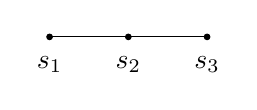
\begin{tikzpicture}
\draw[fill=black] \foreach \x in {1,2,3} {(\x,10) circle (1pt)};
\draw \foreach \x in {1,2,3} {(\x,10) node[label=below:$s_{\x}$]{}};
\draw[-] (1,10) -- (3,10);
\end{tikzpicture}
\caption{Coxeter graph of type $A_3$.}
\end{figure}
\vspace{-1em}
\pause Then $W(A_{3})$ is subject to: \pause 
\begin{itemize}
\item $s_{i}^{2}=1$ for all $i$ \pause
\item $s_{1}s_{2}s_{1}=s_{2}s_{1}s_{2}$, \quad $s_{2}s_{3}s_{2}=s_{3}s_{2}s_{3}$ \pause 
\item $s_{1}s_{3}=s_{3}s_{1}$
\end{itemize}

\pause
\medskip

In this case, $W(A_3)$ is isomorphic to the symmetric group $\Sym_4$ under the correspondence
	\[
	s_1 \leftrightarrow (1\ 2), \quad s_2 \leftrightarrow (2\ 3), \quad s_3 \leftrightarrow (3\ 4).
	\]
\end{block}

\end{frame}

%% -------------------------------------------------------------------

\begin{frame}{\textbf{Type $B$}}\pause

\begin{block}{Example}
The Coxeter group of type $B_4$ is defined by the graph below.
\begin{figure}
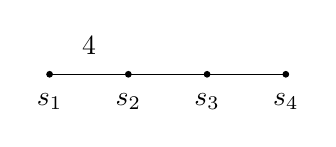
\begin{tikzpicture}
\draw[fill=black] \foreach \x in {1,2,3,4} {(\x,10) circle (1pt)};
\draw \foreach \x in {1,2,3,4} {(\x,10) node[label=below:$s_{\x}$]{}};
\draw[-] (1,10) -- (4,10);
\draw {(1.5,10) node[label=above:$4$]{}};
\end{tikzpicture}
\caption{Coxeter graph of type $B_4$.}
\end{figure}
\vspace{-1em}
\pause Then $W(B_{4})$ is subject to: \pause 
\begin{itemize}
\item $s_{i}^{2}=1$ for all $i$ \pause
\item $s_{2}s_{3}s_{2}=s_{3}s_{2}s_{3}, \quad s_{3}s_{4}s_{3}=s_{4}s_{3}s_{4}$ \pause 
\item $s_{1}s_{2}s_{1}s_{2}=s_{2}s_{1}s_{2}s_{1}$ \pause
\item Non-connected nodes commute
\end{itemize}

\pause
\medskip

In this case, $W(B_4)$ is isomorphic to the group that rearranges and flips 3 coins. %($\Sym_{3}\wreath \mathbb{Z}_{2}$).
\end{block}

\end{frame}

%% -------------------------------------------------------------------

\begin{frame}{\textbf{Type $F$}}\pause

\begin{block}{Example}
The Coxeter group of type $F_5$ is defined by the graph below.
\begin{figure}
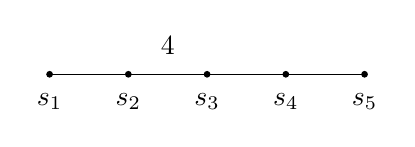
\begin{tikzpicture}
\draw[fill=black] \foreach \x in {1,2,3,4,5} {(\x,10) circle (1pt)};
\draw \foreach \x in {1,2,3} {(\x,10) node[label=below:$s_{\x}$]{}};
\draw {(4,10) node[label=below:$s_{4}$]{}};
\draw {(5,10) node[label=below:$s_{5}$]{}};
\draw {(2.5,10) node[label=above:$4$]{}};
\draw[-] (1,10) -- (5,10);
\end{tikzpicture}
\end{figure}
\vspace{-1em}
\pause Then $W(F_{5})$ is subject to: \pause 
\begin{itemize}
\item $s_{i}^{2}=1$ for all $i$ \pause
\item $s_{1}s_{2}s_{1}=s_{2}s_{1}s_{2}$; \quad $s_{3}s_{4}s_{3}=s_{4}s_{3}s_{4}$; \quad$s_{4}s_{5}s_{4}=s_{5}s_{4}s_{5}$ \pause 
\item $s_{2}s_{3}s_{2}s_{3}=s_{3}s_{2}s_{3}s_{2}$ \pause
\item Non-connected nodes commute
\end{itemize}

\medskip

\pause $F_{4}$ is a finite group, however $F_{n}$ for $n \geq  5$ is an infinite group.
\end{block}

\end{frame}

%% -------------------------------------------------------------------

\begin{frame}{\textbf{Reduced expressions \& Matsumoto's theorem}} \pause

\begin{block}{Definition}
A word $s_{x_1}s_{x_2}\cdots s_{x_m}\in S^{*}$ is called an \alert{expression} for $w\in W$ if it is equal to $w$ when considered as a group element. If $m$ is minimal, it is a \alert{reduced expression}.
\end{block}

\pause
    
\begin{block}{Example}
Consider the expression $s_1s_3s_2s_1s_2$ for an element $w\in W(A_3)$. \pause Note that
	\[
    s_1s_3{\color{red}s_2s_1s_2}={\color{red}s_1s_3}s_1s_2s_1=s_3{\color{red}s_1s_1}s_2s_1=s_3s_2s_1. \pause
    \]
Therefore, $s_1s_3s_2s_1s_2$ is not reduced.  However, the expression on the right is reduced.
\end{block}

\pause

\begin{theorem}[Matsumoto/Tits]
Any two reduced expressions for $w\in W$ differ by a sequence of braid relations.
\end{theorem}

\end{frame}

%% -------------------------------------------------------------------

\begin{frame}{\textbf{Heaps}}\pause

One way of representing reduced expressions is via \alert{heaps}.  Fix a reduced expression $s_{x_1}s_{x_2}\cdots s_{x_m}$ for $w\in W$ (for any straight line Coxeter graph).  \pause Loosely speaking, the heap for this expression is a set of lattice points, one for each $s_{x_{i}}$, embedded in $\mathbb{N}\times \mathbb{N}$ such that: \pause

\begin{itemize}
\item The node corresponding to $s_{x_{i}}$ has vertical component equal to $n+1-x_{i}$ (smaller numbers at the top), \pause
\item If $i<j$ and $s_{x_{i}}$ does not commute with $s_{x_{j}}$, then $s_{x_{i}}$ occurs to the left of $s_{x_{j}}$.
\end{itemize}

\pause

\begin{block}{Example}
Consider {\color{blue!60}$s_{1}s_{2}s_{3}s_{2}$}, {\color{red}$s_{1}s_{3}s_{2}s_{3}$}, and {\color{red}$s_{3}s_{1}s_{2}s_{3}$}, which are all reduced expressions of the same element in $A_{3}$.  \pause It turns out, there are two distinct heaps:
\begin{columns}
\begin{column}{.4\linewidth}
\begin{center}
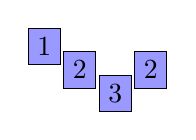
\begin{tikzpicture}[scale=.3]
\node[draw, rectangle, fill=blue!40] at (0,5.5){1};
\node[draw, rectangle, fill=blue!40] at (1.5,4.5){2};
\node[draw, rectangle, fill=blue!40] at (3,3.5){3};
\node[draw, rectangle, fill=blue!40] at (4.5,4.5){2};
\end{tikzpicture}
\end{center}
\end{column}

\begin{column}{.1\linewidth}
\begin{center}
and
\end{center}
\end{column}

\begin{column}{.4\linewidth}
\begin{center}
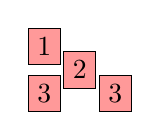
\begin{tikzpicture}[scale=.3]
\node[draw, rectangle, fill=red!40] at (0,5.5){1};
\node[draw, rectangle, fill=red!40] at (0,3.5){3};
\node[draw, rectangle, fill=red!40] at (1.5,4.5){2};
\node[draw, rectangle, fill=red!40] at (3,3.5){3};
\end{tikzpicture}
\end{center}
\end{column}
\end{columns}
\end{block}

\pause

\begin{block}{Comment}
If two reduced expressions differ by a sequence of short braid relations (i.e., commutations), then they have the same heap.
\end{block}

\end{frame}

%% -------------------------------------------------------------------

\begin{frame}{\textbf{Property T and T-avoiding}}\pause

\begin{block}{Definition}
We say that $w\in W$ has \alert{Property T} iff some reduced expression begins or ends with a product of non-commuting generators.  \pause That is,
\begin{columns}
\begin{column}{.4\linewidth}
\begin{center}
$w=\begin{tabular}{c}
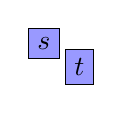
\begin{tikzpicture}[scale=.3]
\node[draw, rectangle, fill=blue!40] at (0,5.5){$s$};
\node[draw, rectangle, fill=blue!40] at (1.5,4.5){$t$};
\end{tikzpicture}
\end{tabular}
({\color{brown}\text{other crap}})$
\end{center}
\end{column}

\begin{column}{.1\linewidth}
\begin{center}
or
\end{center}
\end{column}

\begin{column}{.4\linewidth}
\begin{center}
$w=({\color{brown}\text{other crap}})\begin{tabular}{c}
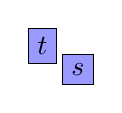
\begin{tikzpicture}[scale=.3]
\node[draw, rectangle, fill=blue!40] at (0,5.5){$t$};
\node[draw, rectangle, fill=blue!40] at (1.5,4.5){$s$};
\end{tikzpicture}
\end{tabular}$
\end{center}
\end{column}
\end{columns}
\end{block}

\pause

\begin{block}{Definition}
We say that $w$ is \alert{T-avoiding} iff $w$ does not have Property T.
\end{block}

\pause

\begin{proposition}
Products of commuting generators are T-avoiding.
\end{proposition}

\pause

\begin{question}
Are there other elements besides products of commuting generators that are T-avoiding?
\end{question}

\end{frame}

%% -------------------------------------------------------------------

\begin{frame}{\textbf{T-avoiding in types $A$, $B$, $\widetilde{C}$, and $D$}}\pause

\begin{block}{Definition}
An element is classified as \alert{bad} iff it is T-avoiding, but \emph{not} a product of commuting generators.
\end{block}

\pause

\begin{theorem}[Cormier, Ernst, Goldenberg, Kelly, Malbon]
In types $A$ and $B$, there are no bad elements. In other words, $w\in W$ is T-avoiding iff $w$ is a product of commuting generators.
\end{theorem}

\pause

\begin{block}{Comment}
The answer isn't so simple in other Coxeter groups.  In particular, there are bad elements in types $\widetilde{C}$ (Ernst) and $D$ (Tyson Gern).
\end{block}
\end{frame}

%% -------------------------------------------------------------------

\begin{frame}{\textbf{Bowties, M's, and Seagulls}}\pause

\begin{proposition}[Cross, Ernst, Hills-Kimball, Quaranta]
The following reduced expressions are bad elements in $F_{5}$: \pause
\end{proposition}

\vspace{1em}

\begin{tabular}{ccc}
\alert{Bowtie} & \alert{M} & \alert{Seagull}\\
\\ \pause
\begin{tabular}{c}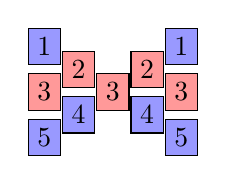
\begin{tikzpicture}[scale=.29]
\node[draw, rectangle, fill=blue!40] at (0,5.5){1};
\node[draw, rectangle, fill=red!40] at (0,3.5){3};
\node[draw, rectangle, fill=blue!40] at (0,1.5){5};
\node[draw, rectangle, fill=red!40] at (1.5,4.5){2};
\node[draw, rectangle, fill=blue!40] at (1.5,2.5){4};
\node[draw, rectangle, fill=red!40] at (3,3.5){3};
\node[draw, rectangle, fill=red!40] at (4.5,4.5){2};
\node[draw, rectangle, fill=blue!40] at (4.5,2.5){4};
\node[draw, rectangle, fill=blue!40] at (6,5.5){1};
\node[draw, rectangle, fill=red!40] at (6,3.5){3};
\node[draw, rectangle, fill=blue!40] at (6,1.5){5};
\end{tikzpicture}
\end{tabular} & \pause
\begin{tabular}{c}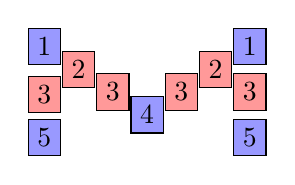
\begin{tikzpicture}[scale=.29]
\node[draw, rectangle, fill=blue!40] at (0,5.5){1};
\node[draw, rectangle, fill=red!40] at (0,3.4){3};
\node[draw, rectangle, fill=blue!40] at (0,1.5){5};
\node[draw, rectangle, fill=red!40] at (1.5,4.5){2};
\node[draw, rectangle, fill=red!40] at (3,3.5){3};
\node[draw, rectangle, fill=blue!40] at (4.5,2.5){4};
\node[draw, rectangle, fill=red!40] at (6,3.5){3};
\node[draw, rectangle, fill=red!40] at (7.5,4.5){2};
\node[draw, rectangle, fill=blue!40] at (9,5.5){1};
\node[draw, rectangle, fill=red!40] at (9,3.5){3};
\node[draw, rectangle, fill=blue!40] at (9,1.5){5};
\end{tikzpicture}
\end{tabular} & \pause 
\begin{tabular}{c}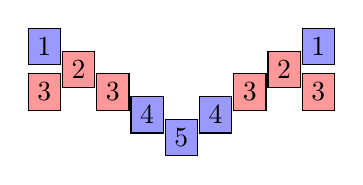
\begin{tikzpicture}[scale=.29]
\node[draw, rectangle, fill=blue!40] at (0,5.5){1};
\node[draw, rectangle, fill=red!40] at (0,3.5){3};
\node[draw, rectangle, fill=red!40] at (1.5,4.5){2};
\node[draw, rectangle, fill=red!40] at (3,3.5){3};
\node[draw, rectangle, fill=blue!40] at (4.5,2.5){4};
\node[draw, rectangle, fill=blue!40] at (6,1.5){5};
\node[draw, rectangle, fill=blue!40] at (7.5,2.5){4};
\node[draw, rectangle, fill=red!40] at (9,3.5){3};
\node[draw, rectangle, fill=red!40] at (10.5,4.5){2};
\node[draw, rectangle, fill=blue!40] at (12,5.5){1};
\node[draw, rectangle, fill=red!40] at (12,3.5){3};
\end{tikzpicture}
\end{tabular}
\end{tabular}

\pause
\vspace{1em}

\emph{We can convert Bowties $\leftrightarrow$ M's $\leftrightarrow$ Seagulls via braid relations. These expressions represent the same group element. We will restrict our attention to the bowties.  We can also stack bowties to create infinitely many bad elements in $F_{5}$.} \pause

\begin{center}
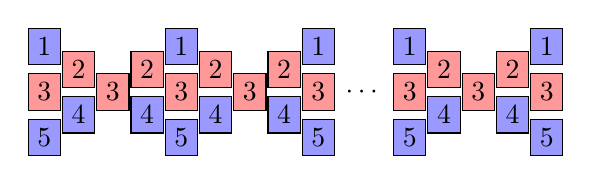
\begin{tikzpicture}[scale=.29]
\node[draw, rectangle, fill=blue!40] at (0,5.5){1};
\node[draw, rectangle, fill=red!40] at (0,3.5){3};
\node[draw, rectangle, fill=blue!40] at (0,1.5){5};
\node[draw, rectangle, fill=red!40] at (1.5,4.5){2};
\node[draw, rectangle, fill=blue!40] at (1.5,2.5){4};
\node[draw, rectangle, fill=red!40] at (3,3.5){3};
\node[draw, rectangle, fill=red!40] at (4.5,4.5){2};
\node[draw, rectangle, fill=blue!40] at (4.5,2.5){4};
\node[draw, rectangle, fill=blue!40] at (6,5.5){1};
\node[draw, rectangle, fill=red!40] at (6,3.5){3};
\node[draw, rectangle, fill=blue!40] at (6,1.5){5};

\node[draw, rectangle, fill=red!40] at (7.5,4.5){2};
\node[draw, rectangle, fill=blue!40] at (7.5,2.5){4};
\node[draw, rectangle, fill=red!40] at (9,3.5){3};
\node[draw, rectangle, fill=red!40] at (10.5,4.5){2};
\node[draw, rectangle, fill=blue!40] at (10.5,2.5){4};
\node[draw, rectangle, fill=blue!40] at (12,5.5){1};
\node[draw, rectangle, fill=red!40] at (12,3.5){3};
\node[draw, rectangle, fill=blue!40] at (12,1.5){5};

\node[] at (14,3.5){$\cdots$};

\node[draw, rectangle, fill=blue!40] at (16,5.5){1};
\node[draw, rectangle, fill=red!40] at (16,3.5){3};
\node[draw, rectangle, fill=blue!40] at (16,1.5){5};
\node[draw, rectangle, fill=red!40] at (17.5,4.5){2};
\node[draw, rectangle, fill=blue!40] at (17.5,2.5){4};
\node[draw, rectangle, fill=red!40] at (19,3.5){3};
\node[draw, rectangle, fill=red!40] at (20.5,4.5){2};
\node[draw, rectangle, fill=blue!40] at (20.5,2.5){4};
\node[draw, rectangle, fill=blue!40] at (22,5.5){1};
\node[draw, rectangle, fill=red!40] at (22,3.5){3};
\node[draw, rectangle, fill=blue!40] at (22,1.5){5};

\end{tikzpicture}
\end{center}

\end{frame}

%% -------------------------------------------------------------------

\begin{frame}{\textbf{Results}}\pause

\begin{theorem}[Cross, Ernst, Hills-Kimball, Quaranta]
An element is T-avoiding in $F_{5}$ iff it is a product of commuting generators or a stack of bowties. 
\end{theorem}

\pause

\begin{block}{Sketch of Proof}
$(\Leftarrow)$ Easy. 

$(\Rightarrow)$ Hard.  Here's an outline. \pause

\begin{itemize}

\item Every bad element must begin or end with $135$ or $13$. \pause

\item If $w$ is bad, then $w$ begins and ends with a bowtie, M, or seagull.

%\item Let $b=\begin{tabular}{c}
%\begin{tikzpicture}[scale=.3]
%\node[draw, rectangle, fill=blue!40] at (0,5.5){1};
%\node[draw, rectangle, fill=red!40] at (0,3.5){3};
%\node[draw, rectangle, fill=blue!40] at (0,1.5){5};
%\node[draw, rectangle, fill=red!40] at (1.5,4.5){2};
%\node[draw, rectangle, fill=blue!40] at (1.5,2.5){4};
%\node[draw, rectangle, fill=red!40] at (3,3.5){3};
%\node[draw, rectangle, fill=red!40] at (4.5,4.5){2};
%\node[draw, rectangle, fill=blue!40] at (4.5,2.5){4};
%\end{tikzpicture}
%\end{tabular}$.  If $\alert{w}=b^{k}\underbrace{\begin{tabular}{c}
%\begin{tikzpicture}[scale=.3]
%\node[draw, rectangle, fill=blue!40] at (6,5.5){1};
%\node[draw, rectangle, fill=red!40] at (6,3.5){3};
%\node[draw, rectangle, fill=blue!40] at (6,1.5){5};
%\end{tikzpicture}
%\end{tabular}\alert{t}}_{\alert{f}}$\ is bad, then $f$ is bad, as well. \pause
%
%\begin{itemize}
%\item[{\LARGE $\hookrightarrow$}] We proved the contrapositive: If $f$ has Property T, then $w$ also has Property T.
%\end{itemize}

\end{itemize}

\end{block}

\end{frame}

%% -------------------------------------------------------------------

\begin{frame}{\textbf{Results}}

\begin{center}
\includegraphics[height=3in]{ChristiesPoster.png}
\end{center}

\end{frame}


%% -------------------------------------------------------------------

\begin{frame}{\textbf{Results}}

\begin{theorem}[Cross, Ernst, Hills-Kimball, Quaranta]
An element is T-avoiding in $F_{5}$ iff it is a product of commuting generators or a stack of bowties. 
\end{theorem}

\begin{block}{Sketch of Proof}
$(\Leftarrow)$ Easy. 

$(\Rightarrow)$ Hard.  Here's an outline.

\begin{itemize}

\item Every bad element must begin or end with $135$ or $13$.

\item If $w$ is bad, then $w$ begins and ends with a bowtie, M, or seagull.\pause

\item Let $b=\begin{tabular}{c}
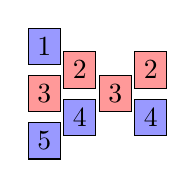
\begin{tikzpicture}[scale=.3]
\node[draw, rectangle, fill=blue!40] at (0,5.5){1};
\node[draw, rectangle, fill=red!40] at (0,3.5){3};
\node[draw, rectangle, fill=blue!40] at (0,1.5){5};
\node[draw, rectangle, fill=red!40] at (1.5,4.5){2};
\node[draw, rectangle, fill=blue!40] at (1.5,2.5){4};
\node[draw, rectangle, fill=red!40] at (3,3.5){3};
\node[draw, rectangle, fill=red!40] at (4.5,4.5){2};
\node[draw, rectangle, fill=blue!40] at (4.5,2.5){4};
\end{tikzpicture}
\end{tabular}$.  If $\alert{w}=b^{k}\underbrace{\begin{tabular}{c}
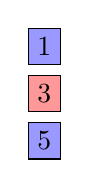
\begin{tikzpicture}[scale=.3]
\node[draw, rectangle, fill=blue!40] at (6,5.5){1};
\node[draw, rectangle, fill=red!40] at (6,3.5){3};
\node[draw, rectangle, fill=blue!40] at (6,1.5){5};
\end{tikzpicture}
\end{tabular}\alert{t}}_{\alert{f}}$\ is bad, then $f$ is bad, as well. \pause

\begin{itemize}
\item[{\LARGE $\hookrightarrow$}] We proved the contrapositive: If $f$ has Property T, then $w$ also has Property T.
\end{itemize}

\end{itemize}

\end{block}

\end{frame}

%% -------------------------------------------------------------------


\begin{frame}{\textbf{Results (continued)}}\pause

\begin{corollary}[Cross, Ernst, Hills-Kimball, Quaranta]
There are no bad elements in $F_{4}$.  That is, the only T-avoiding elements in $F_{4}$ are products of commuting generators.
\end{corollary}

\pause

\begin{conjecture}
An element is T-avoiding in $F_{n}$ for $n\geq 5$ iff it is a product of commuting generators or a stack of bowties times products of commuting generators.  In other words, there are no new bad elements in $F_{n}$ for $n\geq 6$.
\end{conjecture}

\vspace{1em}
\pause

\begin{center}
{\Huge \color{brown}{THANK YOU!}}
\end{center}

\end{frame}

%% -------------------------------------------------------------------  
\end{document}
